% Time-stamp: <2025-05-15 01:26:31 okumura>
\documentclass{jarticle}

\usepackage{tam}
\usepackage{fleqn}
\usepackage{url}
\usepackage{bm}
\usepackage[dvipdfmx]{graphicx}
\usepackage[dvipdfmx]{color}
%\usepackage{color}
\usepackage{colordef}
\usepackage{amssymb}
\usepackage{pdfpages}
\usepackage{ulem}

%%%%%%%%%% Command alias %%%%%%%%%%
\newcommand{\IB}{$\bullet$}
\newcommand{\IC}{$\circ$}
\newcommand{\IS}{$*$}
%%%%%%%%%%%%%%%%%%%%%%%%%%%%%%%%%%%

\title{買電と自己託送を考慮した電力運用最適化モデル}
\author{神戸大学大学院 奥村侑真}
\date{}

\def\baselinestretch{1.02}
\renewcommand{\thefootnote}{\roman{footnote}}

\begin{document}
\maketitle

\section{はじめに}
図\ref{fig:tecseed}に示す電力ネットワークに対する，電力クラスタの電力運
用最適化モデルを示す．

\begin{figure}[h]
 \centering
 
\includegraphics[width=155mm]{../tecseed.pdf}
 \caption{テクシード構成図}
 \label{fig:tecseed}
\end{figure}

\section{準備}

基本要素およびそのスペックを表す定数(\IB を付して記す)と状態変数(\IC を付
して表す)として以下のものを用意する．

%\begin{itemize}
% \item[$\triangleright$] 電力クラスタC$_{i}$ $(i=1,\ldots,N)$:
\begin{itemize}
 \item[\IS] 期T$_k$ ($k=1,\ldots,K$)．本検証では各期の幅($\Delta$)は$60$秒としている．
 \item[\IS] 太陽光発電機G
 \item[\IS] 消費機器D$^{\rm A}$
 \item[\IS] 消費機器D$^{\rm B}$
 \item[\IS] 消費機器D$^{\rm C}$
 \item[\IS] 消費機器（テクシード本社工場）D$^{\rm D}$
   \begin{itemize}
   \item[\IB] 本社工場が必要とする電力 $d^{\rm D}$
   \item[\IB] 本社工場へ託送することのインセンティブ係数 $p^{\rm D}_{k}$   
  \end{itemize} 
 \item[\IS] 固定バッテリーB$^{\rm F}$
  \begin{itemize}
   \item[\IB] 固定バッテリーの容量 $\overline{b}$
  \end{itemize}
 \item[\IS] 電力変換器(太陽光) E$^{\rm P}$
  \begin{itemize}
   \item[\IB] 変換効率 $\alpha^{\rm P}$

  \end{itemize}
 \item[\IS] 電力変換器(系統電力) E$^{\rm S}$
 \item[\IS] 電力変換器(消費機器A) E$^{\rm DA}$
  \begin{itemize}
   \item[\IB] 変換効率 $\alpha^{\rm DA}$
  \end{itemize}
 \item[\IS] 電力変換器(消費機器B) E$^{\rm DB}$
  \begin{itemize}
   \item[\IB] 変換効率 $\alpha^{\rm DB}$
  \end{itemize}
 \item[\IS] 電力変換器(消費機器C) E$^{\rm DC}$
  \begin{itemize}
   \item[\IB] 変換効率 $\alpha^{\rm DC}$
  \end{itemize}
  \item[\IS] 電力変換器(消費機器D) E$^{\rm DD}$
  \begin{itemize}
   \item[\IB] 変換効率 $\alpha^{\rm DD}$
  \end{itemize} 
 \item[\IS] 電力変換器(固定バッテリー)E$^{\rm BF}$
  \begin{itemize}
   \item[\IB] 充電効率 $\alpha^{\rm FC}$
   \item[\IB] 放電効率 $\alpha^{\rm FD}$
   \item[\IB] 自己放電効率 $\alpha^{\rm FT}$
  %\item[\IB] 単位時間あたりの最大充電電量 $a^{\rm FC}$
  %\item[\IB] 単位時間あたりの最大充放電量 $a^{\rm FD}$
  \end{itemize}
 \item[\IS] 系統電力S
   \begin{itemize}
   \item[\IB] 系統買電単価 $p^{\rm BY}_{k}$
   \item[\IB] 単位時間あたりの最大系統買電量 $a^{\rm BY}$
   %\item[\IB] 系統売電単価 $p^{\rm SL}_{k}$
   %\item[\IB] 単位時間あたりの最大系統売電量 $a^{\rm SL}_{k}$
  \end{itemize}
\end{itemize}

\section{定数・変数 \mbox{\normalsize\rm 
~ (定数を「\IB」，変数を「\IC」を付して記すものとする)}}

 \begin{itemize}
  \item[\IB] 太陽光発電電力量(変換前) $g^{\rm P1}_{k}$
  \item[\IC] 太陽光発電電力量(変換後) $g^{\rm P2}_{k}$
  \item[\IC] ムダ電力量 (太陽光発電出力抑制量)$v_{k}$ \\[-2.5ex]
  %
  \item[\IC] 消費電力A (変換前) $d^{\rm A1}_{k}$
  \item[\IB] 消費電力A (変換後) $d^{\rm A2}_{k}$
  %
  \item[\IC] 消費電力B (変換前) $d^{\rm B1}_{k}$
  \item[\IB] 消費電力B (変換後) $d^{\rm B2}_{k}$
  %
  \item[\IC] 消費電力C (変換前) $d^{\rm C1}_{k}$
  \item[\IB] 消費電力C (変換後) $d^{\rm C2}_{k}$
  %
  \item[\IC] 託送電力D (変換前) $d^{\rm D1}_{k}$
  \item[\IC] 託送電力D (変換後) $d^{\rm D2}_{k}$
  %
  \item[\IB] 固定バッテリーの初期SOC $b^{\rm F}_{0}$
  \item[\IC] 固定バッテリーの(期末の)SOC $b^{\rm F}_{k}$
  \item[\IC] 固定バッテリーの充電量(変換前) $x^{\rm FC1}_{k}$
  \item[\IC] 固定バッテリーの充電量(変換後) $x^{\rm FC2}_{k}$
  \item[\IC] 固定バッテリーの放電量(変換前) $x^{\rm FD1}_{k}$
  \item[\IC] 固定バッテリーの放電量(変換後) $x^{\rm FD2}_{k}$ \\[-2.5ex]

  %
  \item[\IC] 系統買電力量$s^{\rm BY}_{k}$
  %\item[\IC] 系統売電力量$s^{\rm SL}_{k}$
  %\item[\IC] 系統電力量(変換前)$s^{1}_{k}$．
  %\item[\IC] 系統電力量(変換後)$s^{2}_{k}$．
  %\item[\IB] 変換効率$\alpha^{\rm S}$．
  %
 % \end{itemize}
\end{itemize}


\section{数理計画モデル}

前項で示した定数・変数を用いて，電力運用最適化問題の線形計画モデルを示す．
%

\noindent
{\rm Minimize}
\begin{equation}
 \sum_{k=1}^{K} \left( p^{\rm BY}_{k}s^{\rm BY}_{k} - p^{\rm D}_{k}d^{\rm D2}_{k} \right)
 \label{eq:minimize}
\end{equation}

\noindent
{\rm Subject to}
%
\begin{equation}
 g^{\rm P2}_{k} + s^{\rm BY} - s^{\rm SL}_{k}
 - x^{\rm FC1}_{k} + x^{\rm FD2}_{k} 
 - d^{\rm A1}_{k} - d^{\rm B1}_{k} - d^{\rm C1}_{k} - d^{\rm D1}_{k} - v_{k} = 0,
 \hfill
 k=1,\ldots,K
~~
\end{equation}
%
\begin{center} --- $ \cdot $ --- $ \cdot $ --- \end{center}
%
\begin{equation}
 g^{\rm P2}_{k} \le \alpha^{\rm P} g^{\rm P1}_{k} ,
 \hfill
 k=1,\ldots,K
 ~~
 \label{eq:gP1gP2}
\end{equation}
%
\begin{center} --- $ \cdot $ --- $ \cdot $ --- \end{center}
%
\begin{equation}
 d^{\rm A2}_{k} \le \alpha^{\rm DA} d^{\rm A1}_{k} ,
 \hfill
 k=1,\ldots,K
~~
 \label{eq:dA1A2}
\end{equation}
%
\begin{equation}
 d^{\rm B2}_{k} \le \alpha^{\rm DB} d^{\rm B1}_{k},
 \hfill
 k=1,\ldots,K
~~
 \label{eq:dB1B2}
\end{equation}
%
\begin{equation}
 d^{\rm C2}_{k} \le \alpha^{\rm DC} d^{\rm C1}_{k},
 \hfill
 k=1,\ldots,K
~~
 \label{eq:dC1C2}
\end{equation}
%
\begin{equation}
 d^{\rm D2}_{k} \le \alpha^{\rm DD} d^{\rm D1}_{k},
 \hfill
 k=1,\ldots,K
~~
 \label{eq:dD1D2}
\end{equation}
%
\begin{center} --- $ \cdot $ --- $ \cdot $ --- \end{center}
%
\begin{equation}
 x^{\rm FC2}_{k} \le \alpha^{\rm FC}x^{\rm FC1}_{k},
 \hfill
 k=1,\ldots,K
~~
 \label{eq:xFC1FC2}
\end{equation}
%
\begin{equation}
 x^{\rm FD2}_{k} \le \alpha^{\rm FD} x^{\rm FD1}_{k} ,
 \hfill
 k=1,\ldots,K
~~
 \label{eq:FD1FD2}
\end{equation}
%
\begin{equation}
 b^{\rm F}_{k} = \alpha^{\rm FT} b^{\rm F}_{k-1} + x^{\rm FC2}_{k} - x^{\rm FD1}_{k},
 \hfill
 k=1,\ldots,K
~~
\end{equation}
%
\begin{equation}
 b^{\rm F}_{k} \le \overline{b}^{\rm F},
 \hfill
 k=1,\ldots,K
~~
\end{equation}
%
\begin{equation}
 x^{\rm FC2}_{k} \le a^{\rm FC},
 \hfill
 k=1,\ldots,K
~~
\end{equation}
%
\begin{equation}
 x^{\rm FD1}_{k} \le a^{\rm FD},
 \hfill
 k=1,\ldots,K
~~
\end{equation}
%
\begin{center} --- $ \cdot $ --- $ \cdot $ --- \end{center}
%
\begin{equation}
 d^{\rm D2}_{k} \le  d^{\rm D}_{k}
 \hfill
 k=1,\ldots,K
~~
 \label{eq:dD2Max}
\end{equation}
%
\begin{center} --- $ \cdot $ --- $ \cdot $ --- \end{center}
%
\begin{equation}
 \sum_{k'=k}^{k+30-1}s^{\rm BY}_{k'} \le  a^{\rm BY}
 \hfill
 k=1,\ldots,K-30+1
~~
 \label{eq:sMax}
\end{equation}

モデル中の定数・変数と電力クラスタとの関係を図\ref{fig:tecseed}に示す．

\begin{figure}[h]
 \centering
 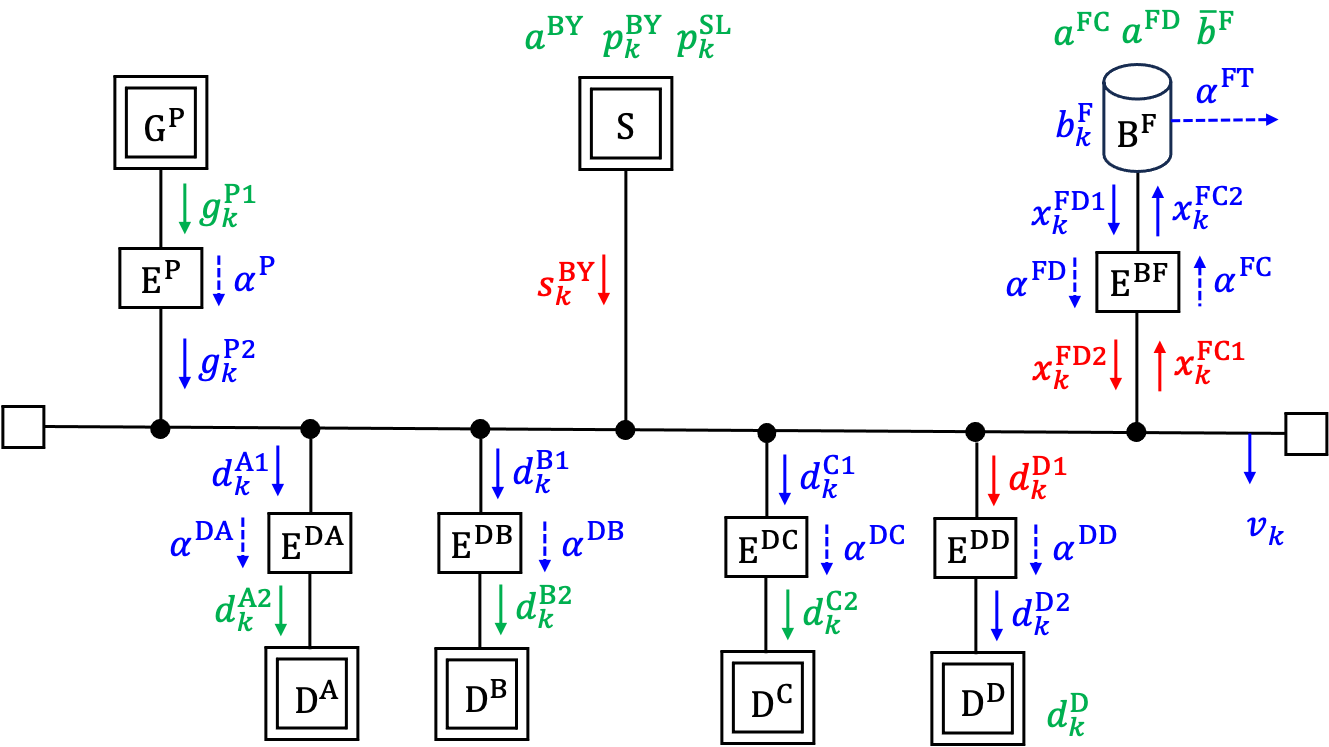
\includegraphics[width=140mm]{../figure/tecseed20250710.png}
 \caption{電力クラスタの構成図 (\textcolor{red}{赤: 決定変数}，\textcolor{blue}{青: 従属変数}，\textcolor{green3}{定数(外生変数)})}
 \label{fig:tecseed}
\end{figure}

\section{買電・自己託送を考慮した，電力運用最適化の検証}
2025年4月17日木曜日から4月26日金曜日までの9日間について検証を行った．4月18日金曜日の午後5時から4月21日月曜日の午前8時までと，4月21日月曜日の午後5時から
4月23日の午前8時までは，テクシード石井工場側が太陽光発電を意図的に停止させていることに留意する．
なお，式(\ref{eq:minimize})における，$p^{\rm BY}_k$の値については，日本卸電力取引所の30分ごとの約定価格のデータ（\url{https://www.jepx.jp/electricpower/market-data/spot/}，2025年6月17日アクセス）を参照して決定した．$p^{\rm D}_k$の値については，十分に小さい値(本検証では0.001)に設定した．これは，託送電力を増やすことよりも買電料金を抑えることを優先するためであり，託送電力を増やすために買電を増やすという挙動を防ぐことを意図している．式(\ref{eq:dD2Max})における$d^{\rm D}_{k}$の値については，まだデータをいただいていないため，ひとまず9:00〜17:00の間は60kW，それ以外の時間帯は0kWになるように値を設定した．さらに，式(\ref{eq:sMax})における$a^{\rm BY}$の値については，神戸大学 共同研究検討依頼資料2025.0516.xlsxを参考に「契約電力が50kW以下にならなければならない」という制約になるように$a^{\rm BY} = \frac{50}{2}$に設定した．

\begin{figure}[h]
 \centering
 
\includegraphics[width=1.1\textwidth, page=1]{Optimization_Results.pdf} % 幅は適宜調整

 \label{fig:optimization_results_p1}
\end{figure}

\begin{figure}[h]
 \centering
 
\includegraphics[width=1.1\textwidth, page=2]{Optimization_Results.pdf} % 幅は適宜調整

 \label{fig:optimization_results_p2}
\end{figure}

\begin{figure}[h]
 \centering
 
\includegraphics[width=1.1\textwidth, page=3]{Optimization_Results.pdf} % 幅は適宜調整
 \caption{最適化結果}
 \label{fig:optimization_results_p3}
\end{figure}



\end{document}
